\documentclass{article}
\input{packages}
\input{acro}
\graphicspath{ {./images/} }

\begin{document}
\input{title}

\cleardoublepage

% TOC %
\pagenumbering{roman}
\tableofcontents
\newpage
\cleardoublepage
\listoffigures
\listoftables
\cleardoublepage
% This is a regular LaTeX comment
\pagenumbering{arabic}
\section{Introduction}


With the growing technological advances, the quantity of healthcare related data produced around the world increased exponentially \cite{choi_generating_2017,henry_adoption_2016}.
With this, the potential for harvesting this data also increases. The value locked within this data could help provide better healthcare with new information about diseases,
drugs, and preventive therapies. It can also help create better health information systems, meaning an overall better clinical practice \cite{ISI:000502534100049}. But for this to happen, the data must reach the capable hands at the right time.
But the release of clinical data has several barriers attached and rightly so. The leakage of patient’s privacy can break the confidence of the population in the healthcare professionals and institutions. Patient safety
and privacy should be kept at all costs and compromise should be kept to minimal values. However, the current mechanisms for privacy maintenance are very long, bureaucratic and time consuming, nationally \cite{comissao_nacional_protecao_de_dados_principios_2015} and internationally \cite{office_for_civil_rights_guidance_2013}. The current scenario and general methods for privacy safeguards are related with pseudo-anonymization techniques.
The removal of certain attributes, identifier modification, code grouping, or discretization are some of the methodologies. But not even these are totally safe \cite{el_emam_systematic_2011}.
Synthetic data appear as an alternative for clinical data sharing, promising great data utility with minimal privacy concerns. Synthetic data is data that is generated automatically through programmatic processes. This is especially impactful for the case at hand since synthetic data has no explicit connection with the original data.\\
This document is aimed for providing a technical overview of a synthetic/real dataset pair and evaluate the synthetically created dataset in terms of utility and privacy.
Not all columns of the original dataset will be assessed, since columns will be filtered by the synthetic columns, since synthesis mechanisms often reduce columns due to identifiers (not needed) and high null columns. \\
This report aims to facilitate the assessment of sharing synthetic data with third parties.

\subsection{ctgan}

\section{Dataset Description}

The final dataset have the variables showed in table \ref{tab:desc}.\\
\begin{longtable}{lll}
\caption{Dataset Variables Description}\label{tab:desc}\\
\toprule
                       Columns &   dtypes &         Type \\
\midrule
\endhead
\midrule
\multicolumn{3}{r}{{Continued on next page}} \\
\midrule
\endfoot

\bottomrule
\endlastfoot
                 IDADE\_MATERNA &  float64 &   Continuous \\
                            GS &   object &  Categorical \\
                  PESO\_INICIAL &  float64 &   Continuous \\
                           IMC &  float64 &   Continuous \\
                      CIGARROS &   object &  Categorical \\
                        ALCOOL &   object &  Categorical \\
               ESTUPEFACIENTES &   object &  Categorical \\
                        A\_PARA &  float64 &  Categorical \\
                       A\_GESTA &  float64 &  Categorical \\
             EUTOCITO\_ANTERIOR &  float64 &  Categorical \\
             VENTOSAS\_ANTERIOR &  float64 &  Categorical \\
              FORCEPS\_ANTERIOR &  float64 &  Categorical \\
           CESARIANAS\_ANTERIOR &  float64 &  Categorical \\
                 TIPO\_GRAVIDEZ &   object &  Categorical \\
                       VIGIADA &   object &  Categorical \\
    NUMERO\_CONSULTAS\_PRE\_NATAL &  float64 &   Continuous \\
              VIGIADA\_HOSPITAL &   object &  Categorical \\
          VIGIADA\_CENTRO\_SAUDE &   object &  Categorical \\
        VIGIADA\_NESTE\_HOSPITAL &   object &  Categorical \\
                 G\_TERAPEUTICA &   object &  Categorical \\
                        NUM\_RN &  float64 &  Categorical \\
                         BACIA &   object &  Categorical \\
         APRESENTACAO\_ADMISSAO &   object &  Categorical \\
                  BISHOP\_SCORE &  float64 &  Categorical \\
    IDADE\_GESTACIONAL\_ADMISSAO &  float64 &   Continuous \\
 TRAB\_PARTO\_ENTRADA\_ESPONTANEO &   object &  Categorical \\
   TRAB\_PARTO\_ENTRADA\_INDUZIDO &   object &  Categorical \\
                           RPM &   object &  Categorical \\
           HIPERTENSAO\_CRONICA &   object &  Categorical \\
       HIPERTENSAO\_GESTACIONAL &   object &  Categorical \\
     HIPERTENSAO\_PRE\_ECLAMPSIA &   object &  Categorical \\
          DIABETES\_GESTACIONAL &   object &  Categorical \\
    DIABETES\_GESTACIONAL\_DIETA &   object &  Categorical \\
 DIABETES\_GESTACIONAL\_INSULINA &   object &  Categorical \\
  DIABETES\_GESTACIONAL\_ANTIBIO &   object &  Categorical \\
              DIABETES\_MATERNA &   object &  Categorical \\
                DIABETES\_TIPO1 &   object &  Categorical \\
                DIABETES\_TIPO2 &   object &  Categorical \\
                  HEMATOLOGICA &   object &  Categorical \\
                  RESPIRATORIA &   object &  Categorical \\
                      CEREBRAL &   object &  Categorical \\
                      CARDIACA &   object &  Categorical \\
                    TIPO\_PARTO &   object &  Categorical \\
         APRESENTACAO\_NO\_PARTO &   object &  Categorical \\
           TRAB\_PARTO\_NO\_PARTO &   object &  Categorical \\
        SEMANAS\_GESTACAO\_PARTO &  float64 &   Continuous \\
                  GRUPO\_ROBSON &   object &  Categorical \\
                DATA\_PARTO\_mes &  float64 &  Categorical \\
                DATA\_PARTO\_ano &  float64 &  Categorical \\
                      COVID\_19 &   object &  Categorical \\
              RETESTE\_NEGATIVO &   object &  Categorical \\
\end{longtable}

\\

The removed columns were:\\
\begin{itemize}
 
  \end{itemize}


\subsection{Brief Variable Overview}
The distribution of the variables is shown in table \ref{tab:realdatadesc}. The values are for numeric data only.\\
\\
\begin{longtable}{lrrrrr}
\caption{Original Data Description}\label{Realdatadesc}\\
\toprule
{} &   mean &  std &    25\% &    50\% &    75\% \\
\midrule
\endhead
\midrule
\multicolumn{6}{r}{{Continued on next page}} \\
\midrule
\endfoot

\bottomrule
\endlastfoot
IDADE\_MATERNA              &   30.6 &  5.7 &   27.0 &   31.0 &   35.0 \\
PESO\_INICIAL               &   65.6 & 13.3 &   56.0 &   63.0 &   73.0 \\
IMC                        &   25.0 &  6.2 &   21.5 &   23.9 &   27.3 \\
A\_PARA                     &    0.7 &  0.8 &    0.0 &    1.0 &    1.0 \\
A\_GESTA                    &    1.4 &  1.5 &    0.0 &    2.0 &    2.0 \\
EUTOCITO\_ANTERIOR          &    0.4 &  0.7 &    0.0 &    0.0 &    1.0 \\
VENTOSAS\_ANTERIOR          &    0.1 &  0.2 &    0.0 &    0.0 &    0.0 \\
FORCEPS\_ANTERIOR           &    0.0 &  0.1 &    0.0 &    0.0 &    0.0 \\
CESARIANAS\_ANTERIOR        &    0.2 &  0.4 &    0.0 &    0.0 &    0.0 \\
NUMERO\_CONSULTAS\_PRE\_NATAL &    6.3 &  5.4 &    2.0 &    4.0 &    9.0 \\
NUM\_RN                     &    1.0 &  0.1 &    1.0 &    1.0 &    1.0 \\
BISHOP\_SCORE               &    4.9 &  3.1 &    3.0 &    4.0 &    7.0 \\
IDADE\_GESTACIONAL\_ADMISSAO &   38.9 &  1.9 &   38.4 &   39.3 &   40.1 \\
SEMANAS\_GESTACAO\_PARTO     &  273.9 & 12.6 &  270.0 &  276.0 &  281.0 \\
DATA\_PARTO\_mes             &    6.7 &  3.3 &    4.0 &    7.0 &   10.0 \\
DATA\_PARTO\_ano             & 2017.8 &  1.5 & 2017.0 & 2018.0 & 2019.0 \\
\end{longtable}

\\
\\
\begin{longtable}{lrrrrr}
\caption{Synthetic Data Description}\label{Synth data desc}\\
\toprule
{} &   mean &  std &    25\% &    50\% &    75\% \\
\midrule
\endhead
\midrule
\multicolumn{6}{r}{{Continued on next page}} \\
\midrule
\endfoot

\bottomrule
\endlastfoot
IDADE\_MATERNA              &   33.9 &  6.1 &   30.0 &   32.0 &   40.0 \\
PESO\_INICIAL               &   60.7 &  8.1 &   57.0 &   62.0 &   64.0 \\
IMC                        &   22.4 &  2.8 &   20.5 &   23.4 &   23.6 \\
A\_PARA                     &    1.0 &  1.0 &    1.0 &    1.0 &    1.0 \\
A\_GESTA                    &    1.5 &  1.7 &    0.0 &    1.0 &    3.0 \\
EUTOCITO\_ANTERIOR          &    0.4 &  0.9 &    0.0 &    0.0 &    0.0 \\
VENTOSAS\_ANTERIOR          &    0.1 &  0.3 &    0.0 &    0.0 &    0.0 \\
FORCEPS\_ANTERIOR           &    0.0 &  0.1 &    0.0 &    0.0 &    0.0 \\
CESARIANAS\_ANTERIOR        &    0.2 &  0.5 &    0.0 &    0.0 &    0.0 \\
NUMERO\_CONSULTAS\_PRE\_NATAL &   10.2 &  7.8 &    4.0 &    8.0 &   17.0 \\
NUM\_RN                     &    1.0 &  0.2 &    1.0 &    1.0 &    1.0 \\
BISHOP\_SCORE               &    4.2 &  1.6 &    4.0 &    4.0 &    4.0 \\
IDADE\_GESTACIONAL\_ADMISSAO &   38.9 &  1.4 &   38.5 &   39.3 &   39.5 \\
SEMANAS\_GESTACAO\_PARTO     &  267.2 & 18.9 &  267.0 &  270.0 &  278.0 \\
DATA\_PARTO\_mes             &    6.8 &  3.3 &    4.0 &    7.0 &   10.0 \\
DATA\_PARTO\_ano             & 2018.1 &  1.6 & 2017.0 & 2018.0 & 2020.0 \\
\end{longtable}

\\
\\
\subsection{Null Overview}

Concerning null/empty cells for each column, the table \ref{tab:nullcomparasion} presents the comparison of the two datasets.\\

\begin{longtable}{lrr}
\caption{Null values Comparison}\label{tab:nullcomparison}\\
\toprule
                        Column &    Real & Synthetic \\
\midrule
\endhead
\midrule
\multicolumn{3}{r}{{Continued on next page}} \\
\midrule
\endfoot

\bottomrule
\endlastfoot
                 IDADE\_MATERNA &       0 &         0 \\
                            GS &    19.0 &      38.0 \\
                  PESO\_INICIAL &  1226.0 &         0 \\
                           IMC &  1571.0 &         0 \\
                      CIGARROS &       0 &         0 \\
                        ALCOOL &       0 &         0 \\
               ESTUPEFACIENTES &       0 &         0 \\
                        A\_PARA &   667.0 &         0 \\
                       A\_GESTA &       0 &         0 \\
             EUTOCITO\_ANTERIOR &       0 &         0 \\
             VENTOSAS\_ANTERIOR &       0 &         0 \\
              FORCEPS\_ANTERIOR &       0 &         0 \\
           CESARIANAS\_ANTERIOR &       0 &         0 \\
                 TIPO\_GRAVIDEZ &   698.0 &    1171.0 \\
                       VIGIADA &     4.0 &      40.0 \\
    NUMERO\_CONSULTAS\_PRE\_NATAL &  1714.0 &         0 \\
              VIGIADA\_HOSPITAL &  1885.0 &    3428.0 \\
          VIGIADA\_CENTRO\_SAUDE &  3624.0 &    2435.0 \\
        VIGIADA\_NESTE\_HOSPITAL &  1964.0 &     987.0 \\
                 G\_TERAPEUTICA &  1555.0 &    1179.0 \\
                        NUM\_RN &       0 &         0 \\
                         BACIA &  5932.0 &    6574.0 \\
         APRESENTACAO\_ADMISSAO &       0 &         0 \\
                  BISHOP\_SCORE &  6129.0 &         0 \\
    IDADE\_GESTACIONAL\_ADMISSAO &    42.0 &         0 \\
 TRAB\_PARTO\_ENTRADA\_ESPONTANEO &       0 &         0 \\
   TRAB\_PARTO\_ENTRADA\_INDUZIDO &       0 &         0 \\
                           RPM &       0 &         0 \\
           HIPERTENSAO\_CRONICA &       0 &         0 \\
       HIPERTENSAO\_GESTACIONAL &       0 &         0 \\
     HIPERTENSAO\_PRE\_ECLAMPSIA &       0 &         0 \\
          DIABETES\_GESTACIONAL &       0 &         0 \\
    DIABETES\_GESTACIONAL\_DIETA &       0 &         0 \\
 DIABETES\_GESTACIONAL\_INSULINA &       0 &         0 \\
  DIABETES\_GESTACIONAL\_ANTIBIO &       0 &         0 \\
              DIABETES\_MATERNA &       0 &         0 \\
                DIABETES\_TIPO1 &       0 &         0 \\
                DIABETES\_TIPO2 &       0 &         0 \\
                  HEMATOLOGICA &       0 &         0 \\
                  RESPIRATORIA &       0 &         0 \\
                      CEREBRAL &       0 &         0 \\
                      CARDIACA &       0 &         0 \\
                    TIPO\_PARTO &       0 &         0 \\
         APRESENTACAO\_NO\_PARTO &       0 &         0 \\
           TRAB\_PARTO\_NO\_PARTO &       0 &         0 \\
        SEMANAS\_GESTACAO\_PARTO &    10.0 &         0 \\
                  GRUPO\_ROBSON &       0 &         0 \\
                DATA\_PARTO\_mes &       0 &         0 \\
                DATA\_PARTO\_ano &       0 &         0 \\
                      COVID\_19 &   935.0 &    1556.0 \\
              RETESTE\_NEGATIVO &  1278.0 &    1042.0 \\
\end{longtable}
\\

For the rest of the reports, when null are removed or imputed, it shall be indicated.
\section{Utility evaluation}\\
This section aims tom assess the quality of the synthetic dataset by assessing the similarities with the original one. The subsection \ref{sec:visual} will be concerned with only visual methods and the following subsection \ref{sec:quant} with numerical comparison.\\
\subsection{Visual}  \label{sec:visual}
This section is about visual methods for assessing the quality of the generated data.\\
\subsubsection{Heatmaps}
Heatmaps are concerning the correlations between all continuous variables. The more figure \ref{fig:heatmapreal} and figure \ref{fig:heatmapsynth} are alike, the more similar are the continuous variables relations between all columns. 

\begin{figure}[h!]
\centering
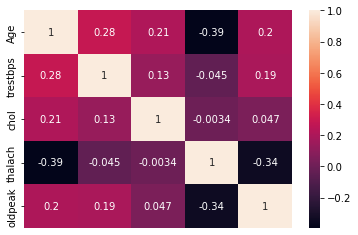
\includegraphics[width=120mm]{heatmap_real}
\caption{Heatmap for Real  Dataset}
\label{fig:heatmapreal}
\end{figure}
\\

\begin{figure}[h!]
\centering
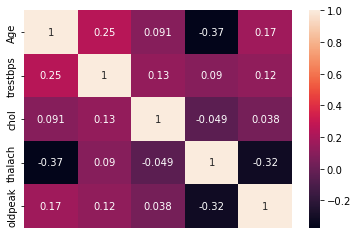
\includegraphics[width=120mm]{heatmap_synth}
\caption{Heatmap for Synthetic Dataset}
\label{fig:heatmapsynth}
\end{figure}

\subsubsection{Plotting Categorical Variables}
Categorical variables will be plotted as count bar plots.

\begin{figure}[H]
\centering
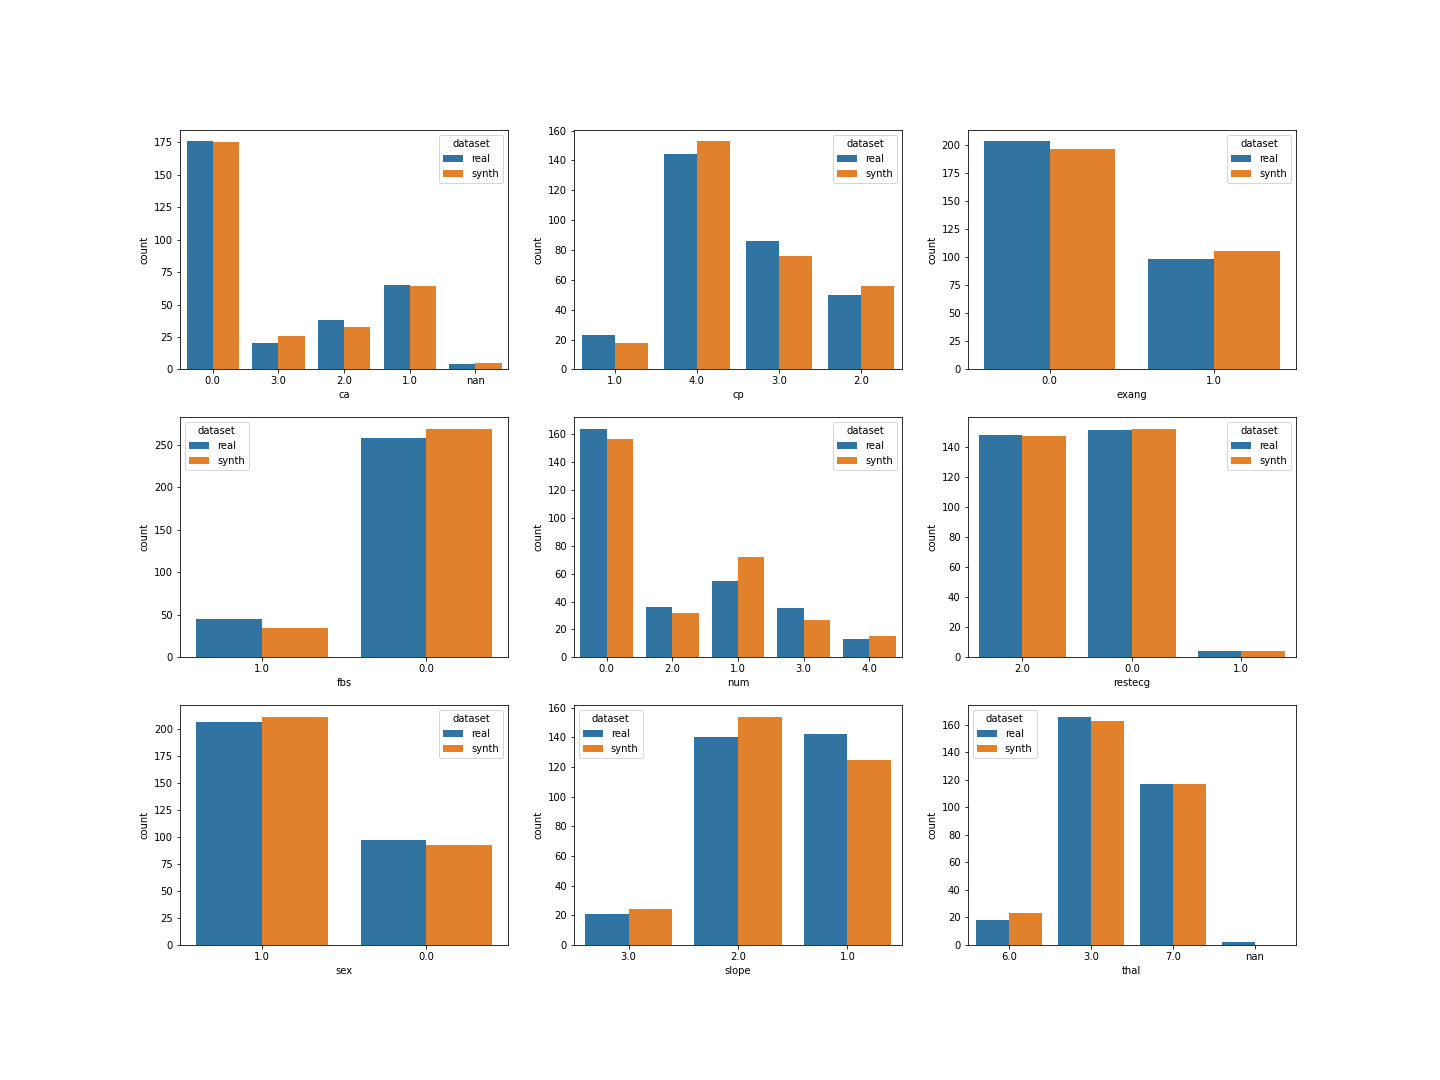
\includegraphics[width=\textwidth]{images/categorical_plot_0.png}
\caption{Categorical Variable Plots 1}
\label{fig:categorical1}
\end{figure}

\begin{figure}[H]
\centering
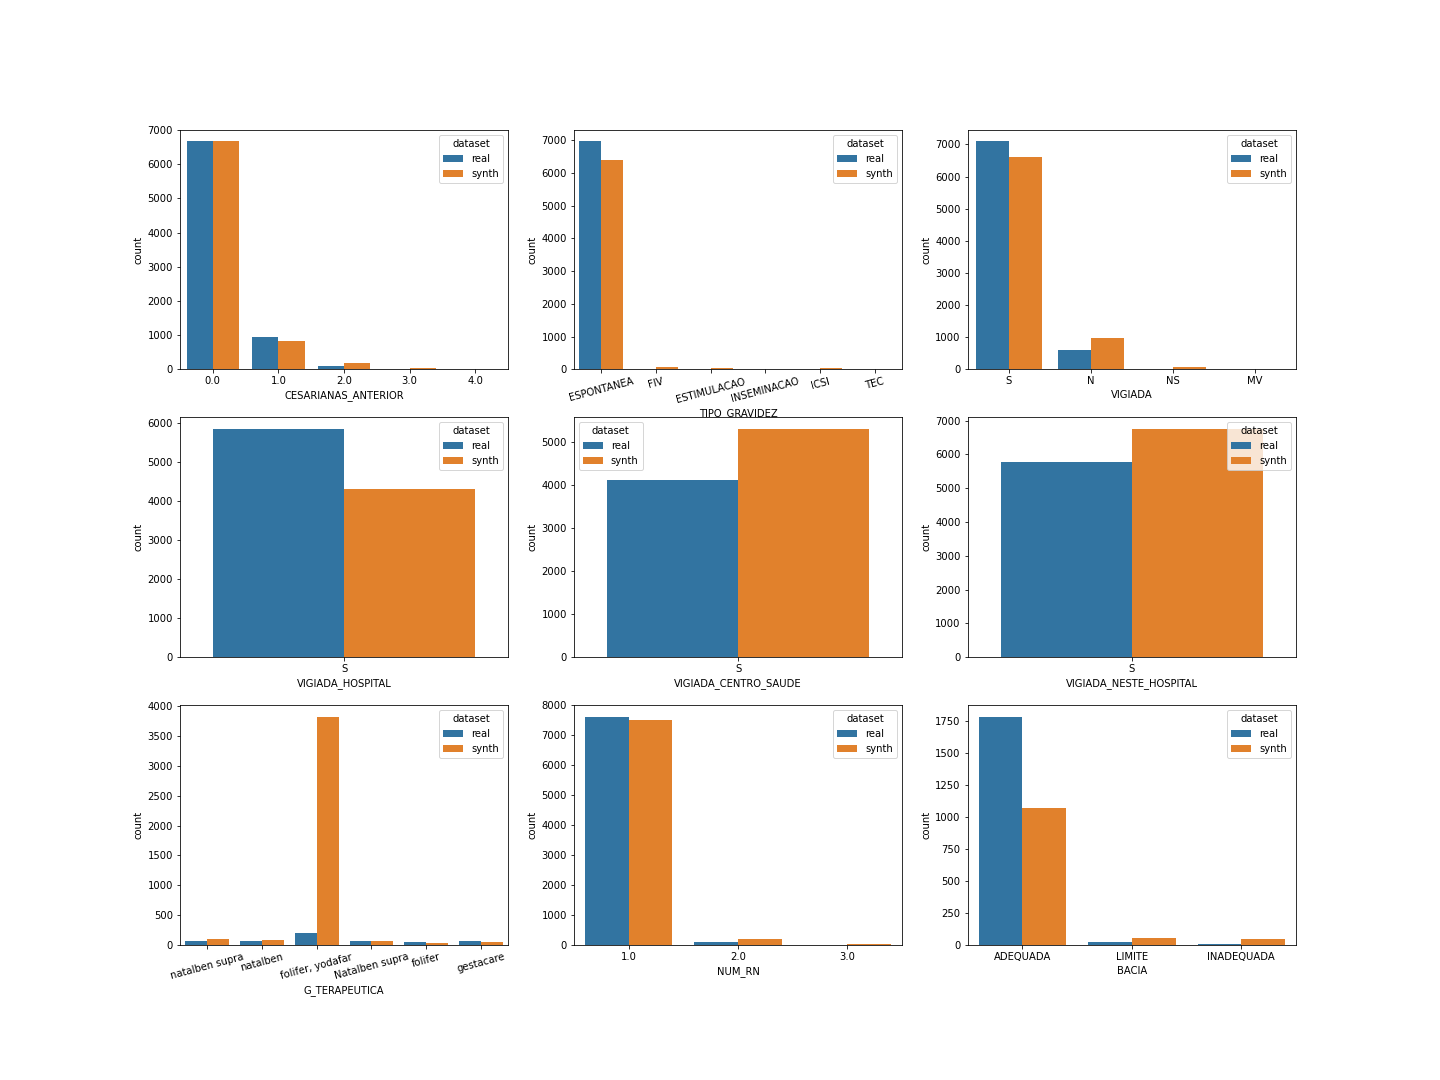
\includegraphics[width=\textwidth]{images/categorical_plot_1.png}
\caption{Categorical Variable Plots 2}
\label{fig:categorical2}
\end{figure}

\begin{figure}[H]
\centering
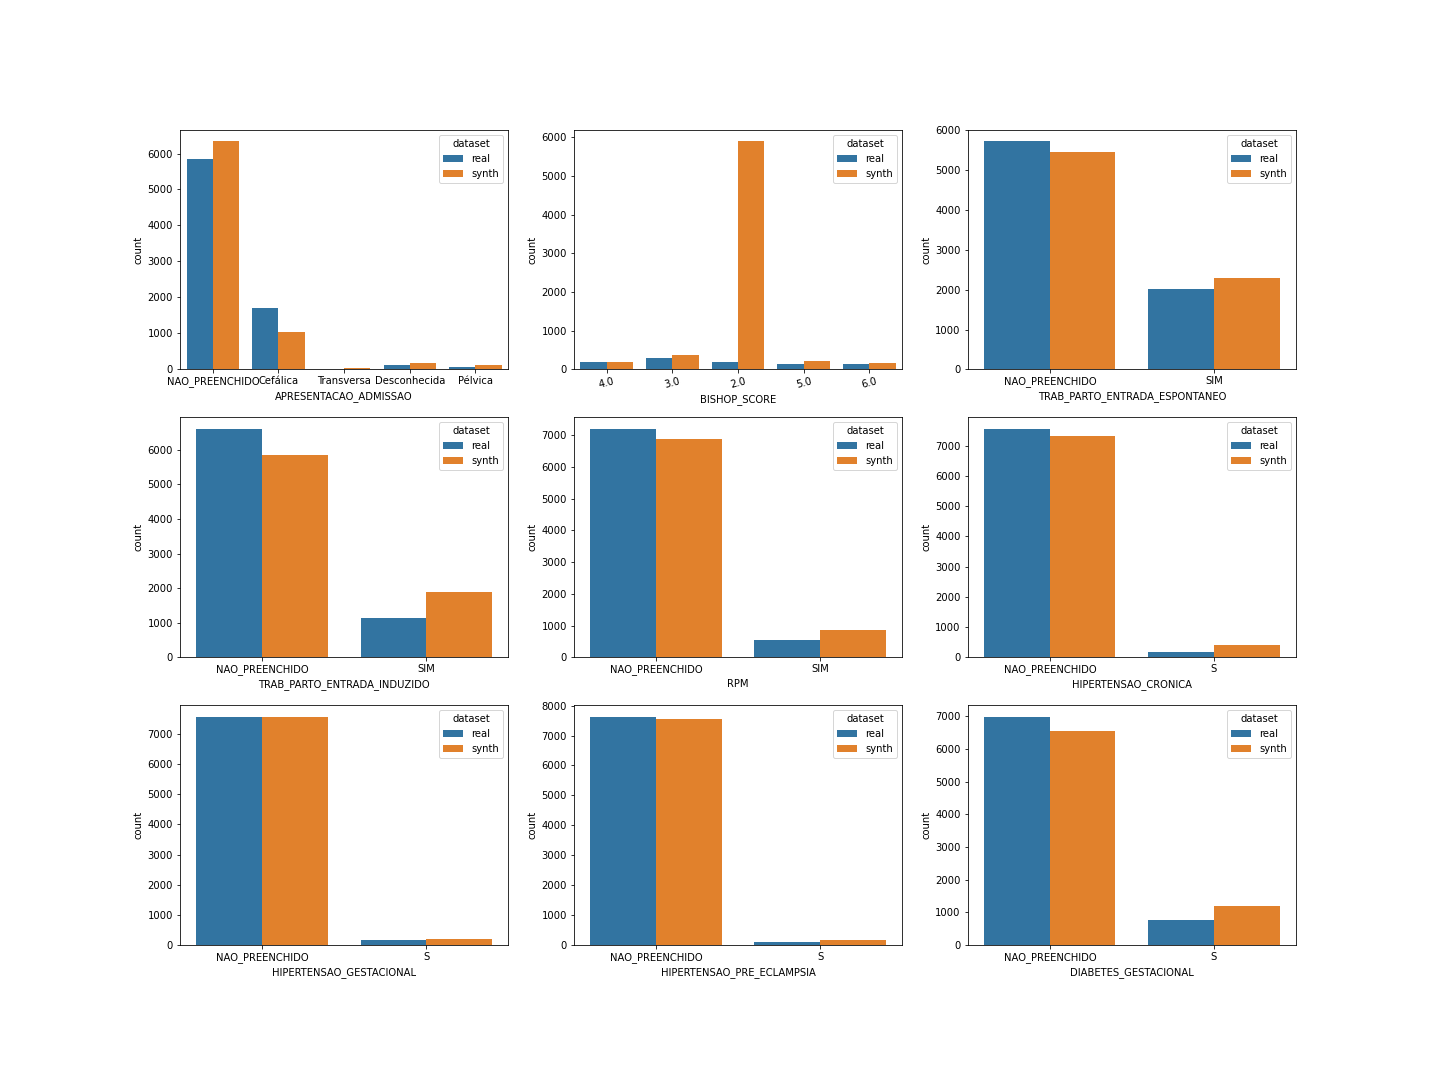
\includegraphics[width=\textwidth]{images/categorical_plot_2.png}
\caption{Categorical Variable Plots 3}
\label{fig:categorical2}
\end{figure}

\begin{figure}[H]
\centering
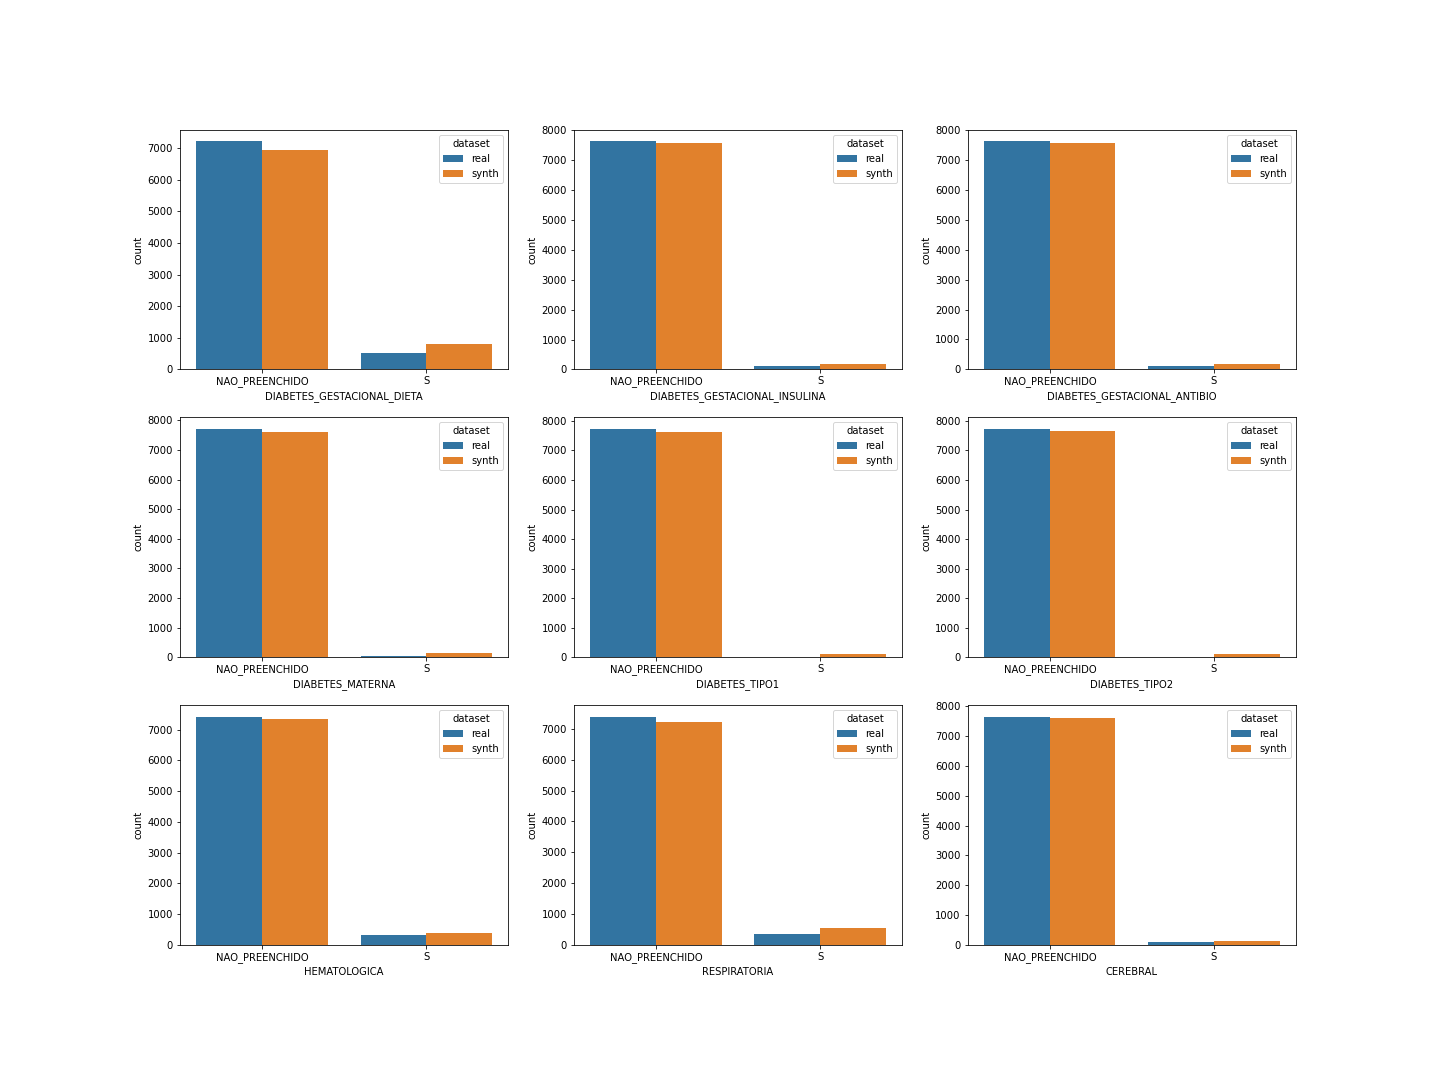
\includegraphics[width=\textwidth]{images/categorical_plot_3.png}
\caption{Categorical Variable Plots 4}
\label{fig:categorical3}
\end{figure}

\begin{figure}[H]
\centering
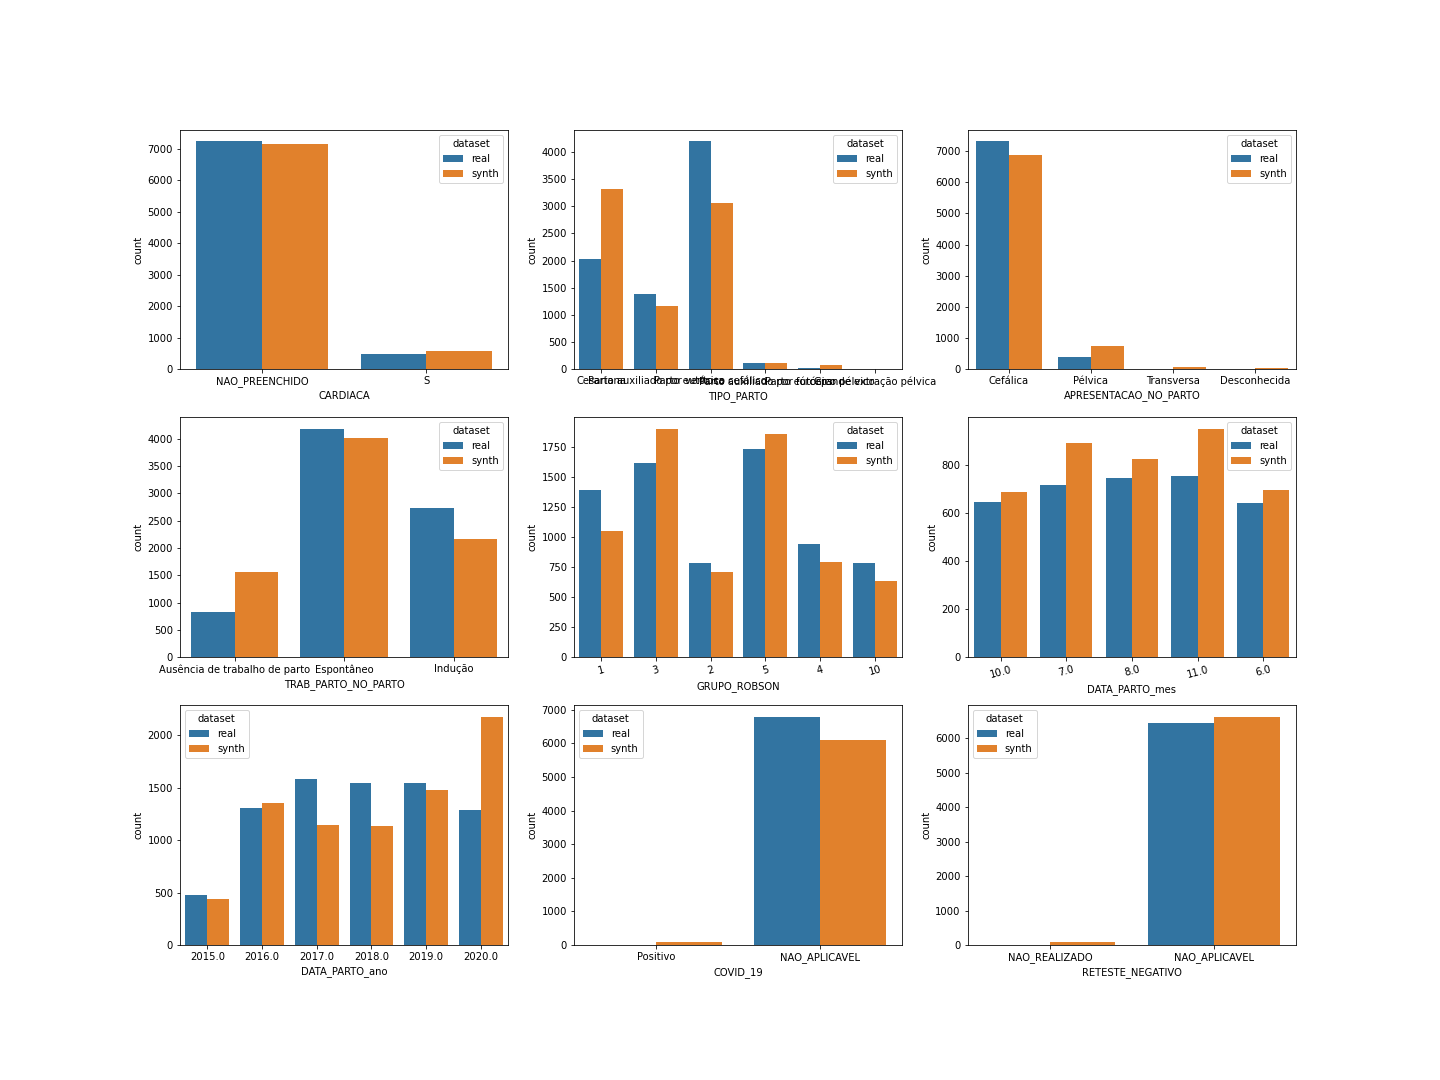
\includegraphics[width=\textwidth]{images/categorical_plot_4.png}
\caption{Categorical Variable Plots 5}
\label{fig:categorical4}
\end{figure}

\subsubsection{Plotting Continuous Variables}
Continuous variables will be plotted as density plots. See figure \ref{fig:continuous}.
\begin{figure}[h!]
\centering
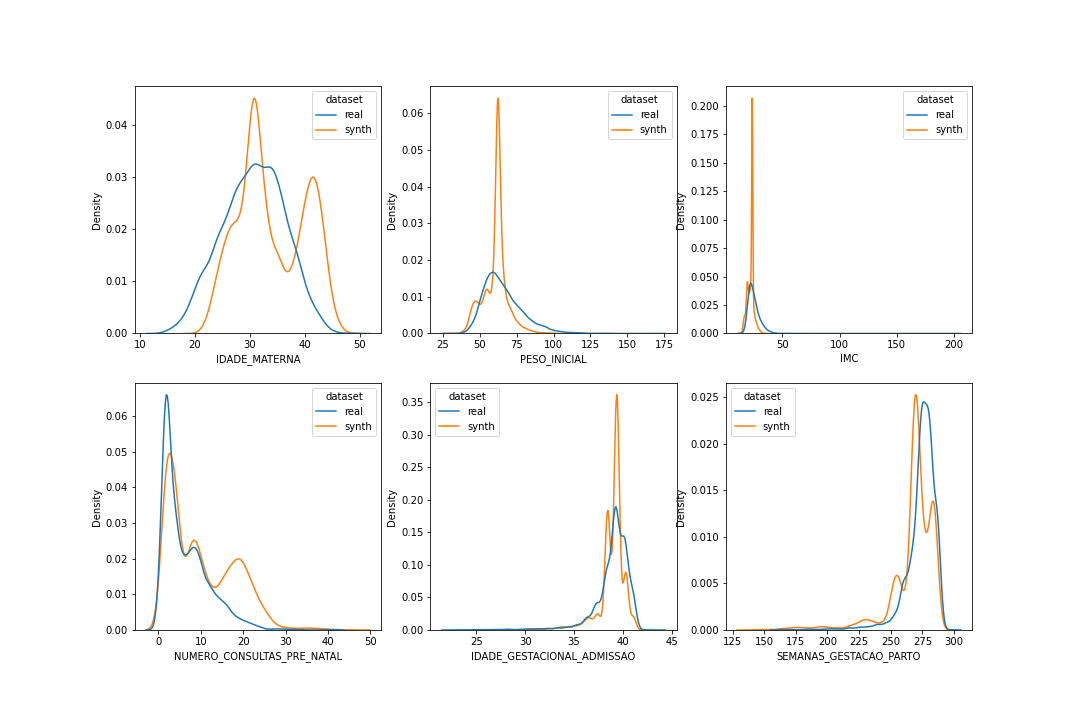
\includegraphics[width=\textwidth]{images/continuous_plot_0.png}
\caption{Categorical Variable Plots}
\label{fig:continuous}
\end{figure}

\subsubsection{Pairplot}

\begin{figure}[H]
\centering
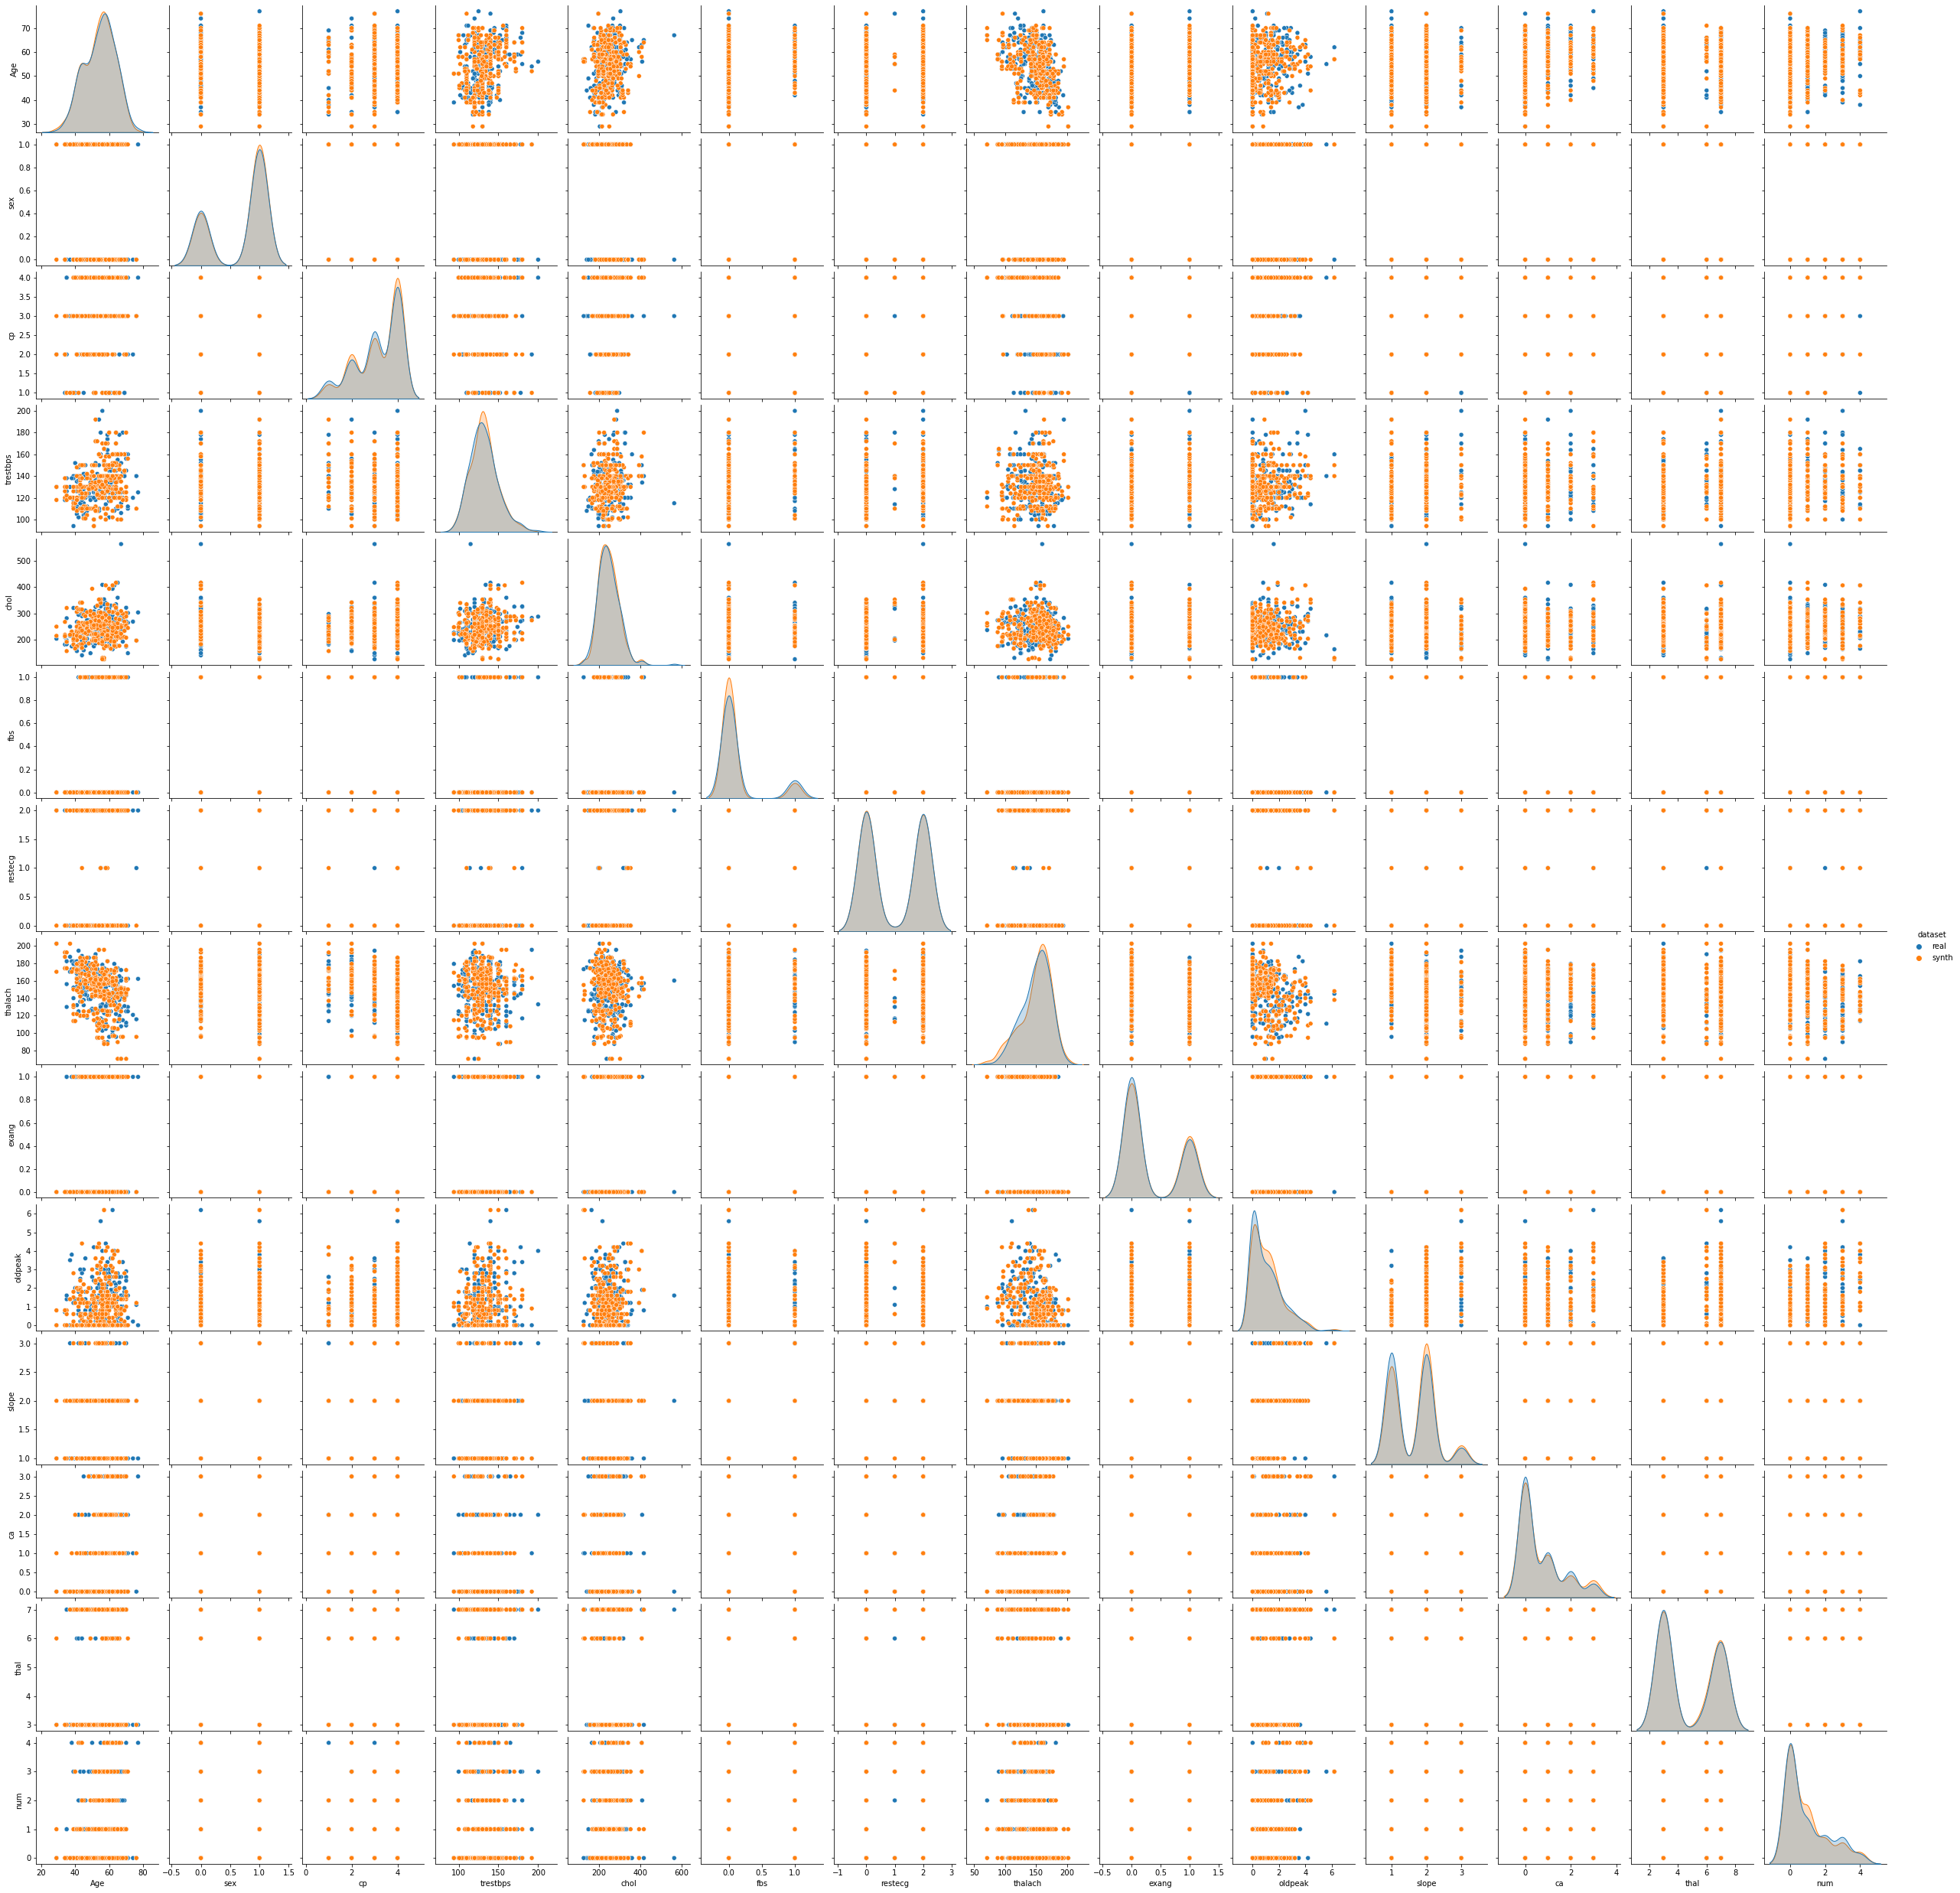
\includegraphics[width=\textwidth]{pairplot}
\caption{PairPlot}
\label{fig:pairplot}
\end{figure}
  
\subsection{Quantitative Evaluation}\label{sec:quant}
This section hopes to bring more efficient methods of assessing the quality of a synthetic dataset. nowadays there are not unanimous metrics regarding this subject. For this reason, several different metrics are presented.\\
Columnwise metrics will assess how similar the equivalent columns are. The tablewise metrics will try to measure how the datasets as a whole are similar.
\subsubsection{Columnwise}
  
\paragraph{Kolmogorov–Smirnov test}
In statistics, the \textit{Kolmogorov–Smirnov} (\acrshort{kstest}) test is a nonparametric test of the equality of continuous, one-dimensional probability distributions that can be used to compare a sample with a reference probability distribution (one-sample K–S test), or to compare two samples (two-sample K–S test). It is named after Andrey Kolmogorov and Nikolai Smirnov. 
The two-sample K–S test is one of the most useful and general nonparametric methods for comparing two samples, as it is sensitive to differences in both location and shape of the empirical cumulative distribution functions of the two samples \cite{kstest_wiki}.  The results for the data are:\\

\begin{longtable}{lr}
\caption{K-S test Results}\label{tab:ks}\\
\toprule
{} & Value \\
\midrule
\endhead
\midrule
\multicolumn{2}{r}{{Continued on next page}} \\
\midrule
\endfoot

\bottomrule
\endlastfoot
IMC                        &  0.75 \\
IDADE\_MATERNA              &  0.77 \\
PESO\_INICIAL               &  0.81 \\
SEMANAS\_GESTACAO\_PARTO     &  0.66 \\
IDADE\_GESTACIONAL\_ADMISSAO &  0.80 \\
NUMERO\_CONSULTAS\_PRE\_NATAL &  0.69 \\
\end{longtable}



\paragraph{Chi-squared test}
This metric uses the chi-squared test to compare the distributions of the two categorical columns. It returns the resulting p-value so that a small value indicates that we can reject the null hypothesis (i.e. and suggests that the distributions are different). So higher p-value, chance of being similar is big, while small value indicates a small chance of being similar.\\

\begin{longtable}{lr}
\caption{Chi-Squared test Results}\label{tab:cs}\\
\toprule
{} & Value \\
\midrule
\endhead
\midrule
\multicolumn{2}{r}{{Continued on next page}} \\
\midrule
\endfoot

\bottomrule
\endlastfoot
ALCOOL                        &  0.89 \\
APRESENTACAO\_ADMISSAO         &  1.00 \\
APRESENTACAO\_NO\_PARTO         &  0.99 \\
A\_GESTA                       &  1.00 \\
A\_PARA                        &  1.00 \\
BACIA                         &  0.99 \\
BISHOP\_SCORE                  &  1.00 \\
CARDIACA                      &  0.96 \\
CEREBRAL                      &  0.97 \\
CESARIANAS\_ANTERIOR           &  1.00 \\
CIGARROS                      &  0.91 \\
COVID\_19                      &  0.94 \\
DATA\_PARTO\_ano                &  1.00 \\
DATA\_PARTO\_mes                &  1.00 \\
DIABETES\_GESTACIONAL          &  0.85 \\
DIABETES\_GESTACIONAL\_ANTIBIO  &  0.94 \\
DIABETES\_GESTACIONAL\_DIETA    &  0.89 \\
DIABETES\_GESTACIONAL\_INSULINA &  0.93 \\
DIABETES\_MATERNA              &  0.82 \\
DIABETES\_TIPO1                &  0.71 \\
DIABETES\_TIPO2                &  0.73 \\
ESTUPEFACIENTES               &  0.75 \\
EUTOCITO\_ANTERIOR             &  1.00 \\
FORCEPS\_ANTERIOR              &  0.95 \\
GRUPO\_ROBSON                  &  1.00 \\
GS                            &  1.00 \\
G\_TERAPEUTICA                 &  1.00 \\
HEMATOLOGICA                  &  0.96 \\
HIPERTENSAO\_CRONICA           &  0.85 \\
HIPERTENSAO\_GESTACIONAL       &  0.99 \\
HIPERTENSAO\_PRE\_ECLAMPSIA     &  0.94 \\
NUM\_RN                        &  0.98 \\
RESPIRATORIA                  &  0.90 \\
RETESTE\_NEGATIVO              &  0.98 \\
RPM                           &  0.87 \\
TIPO\_GRAVIDEZ                 &  1.00 \\
TIPO\_PARTO                    &  1.00 \\
TRAB\_PARTO\_ENTRADA\_ESPONTANEO &  0.93 \\
TRAB\_PARTO\_ENTRADA\_INDUZIDO   &  0.78 \\
TRAB\_PARTO\_NO\_PARTO           &  0.95 \\
VENTOSAS\_ANTERIOR             &  0.99 \\
VIGIADA                       &  1.00 \\
VIGIADA\_CENTRO\_SAUDE          &  0.76 \\
VIGIADA\_HOSPITAL              &  0.64 \\
VIGIADA\_NESTE\_HOSPITAL        &  0.77 \\
\end{longtable}



\paragraph{Distance Metrics}
In mathematical statistics, the \textbf{Kullback–Leibler divergence} ( \acrshort{kl}),  (also called relative entropy), is a measure of how one probability distribution is different from a second, reference probability distribution.\\
In probability theory and statistics, the \textbf{Jensen–Shannon divergence} (\acrshort{jsd}) is a method of measuring the similarity between two probability distributions. It is also known as information radius (IRad) or total divergence to the average.It is based on the Kullback–Leibler divergence, with some notable (and useful) differences, including that it is symmetric and it always has a finite value. The square root of the Jensen–Shannon divergence is a metric often referred to as Jensen-Shannon distance.     
In mathematics, the \textbf{Wasserstein distance} (\acrshort{wass}) or Kantorovich–Rubinstein metric is a distance function defined between probability distributions on a given metric space M.
Intuitively, if each distribution is viewed as a unit amount of earth (soil) piled on M, the metric is the minimum "cost" of turning one pile into the other, which is assumed to be the amount of earth that needs to be moved times the mean distance it has to be moved. Because of this analogy, the metric is known in computer science as the earth mover's distance.
The name "Wasserstein distance" was coined by R. L. Dobrushin in 1970, after the Russian mathematician Leonid Vaseršteĭn who introduced the concept in 1969. Most English-language publications use the German spelling "Wasserstein" (attributed to the name "Vaseršteĭn" being of German origin). The values of different distance metrics are present in the table \ref{tab:distance}.\\

\caption{Distance Metrics Results Aggregated}\label{tab:distance}   
\begin{longtable}{lrrrr}
\caption{Distance Metrics results}\label{tab:distance}\\
\toprule
{} &     min &  average &    max &    std \\
\midrule
\endhead
\midrule
\multicolumn{5}{r}{{Continued on next page}} \\
\midrule
\endfoot

\bottomrule
\endlastfoot
KL      & -0.1349 &   0.0628 & 2.0816 & 0.3131 \\
JSD     &  0.0000 &   0.0780 & 0.5851 & 0.1074 \\
Wass    &  0.0002 &   0.0347 & 0.1993 & 0.0397 \\
Entropy &  0.0000 &   0.0980 & 2.6668 & 0.4156 \\
\end{longtable}

    

\subsubsection{Tablewise}

\paragraph{DiscreteKLDivergence}

The value is 0.57.\\

\paragraph{ContinuousKLDivergence}
The value is 0.658.\\


\paragraph{BNLikelihood}

This metric fits a Bayesian Network to the real data and then evaluates the average likelihood of the rows from the synthetic data on it. 
The value is 3.2947144407064006e-11.\\

\paragraph{BNLogLikelihood}

This metric fits a Bayesian Network to the real data and then evaluates the average log likelihood of the rows from the synthetic data on it.
The value is -18.753750698450673.\\


\paragraph{GMLogLikelihood}

This metric fits multiple Gaussian Mixture models to the real data and then evaluates the average log likelihood of the synthetic data on them.
The value is -24.635189983083592.\\

\paragraph{Coverage Support}
Association rule mining [1,2] is one of the important data mining tasks that is nowadays applied to solve different kinds of problems in weak formalization fields. The main goal of association rule mining is to find all rules in datasets that satisfy some basic requirements, such as minimum support and minimum confidence. It was initially proposed by Agrawal [3] to solve the market basket problem in transactional datasets and now it has developed to solve many other problems, such as classification, clustering, etc. Classification and prediction are two important tasks of data mining that can be used to extract the hidden regularities from the given datasets to form accurate models (classifiers). Classification approaches aim to build classifiers (models) to predict the class label of a future data object. Such analysis can help to provide us with a better understanding of the data comprehensively. Classification methods have been widely used in many real-world applications, such as customer relationship management [4], medical diagnosis [5] and industrial design [6].

\paragraph{Cross-validation}
For this evaluation, we will make cross-validation with several machine-learning algorithms.
The data will be trained on synthetic and then test on real and synthetic. This will help assess how plausible it is to deliver the synthetic data for data analysis. If the test values are similar, the synthetic dataset may be used as a proxy of the real.\\
On the other hand, training on real and testing on real and synthetic will help assess how the synthetic dataset correctly created the relationships between all variables.
For this purpose, there are 3 evaluation metrics, real on real, synthetic on synthetic and cross evaluation. Training with real and testing on synthetic and the other way around. For integer columns, mean absolute error was used, for categorical f1 (macro) was used (multiclass classification).\\

\begin{longtable}{lr}
\caption{Same Dataset score}\label{tab:samedatascore}\\
\toprule
{} &     0 \\
\midrule
\endhead
\midrule
\multicolumn{2}{r}{{Continued on next page}} \\
\midrule
\endfoot

\bottomrule
\endlastfoot
IDADE\_MATERNA                 &  0.76 \\
GS                            &  1.00 \\
PESO\_INICIAL                  &  0.82 \\
IMC                           &  0.63 \\
CIGARROS                      &  0.99 \\
ALCOOL                        &  0.95 \\
ESTUPEFACIENTES               &  0.96 \\
A\_PARA                        &  5.72 \\
A\_GESTA                       &  3.93 \\
EUTOCITO\_ANTERIOR             &  5.00 \\
VENTOSAS\_ANTERIOR             &  1.90 \\
FORCEPS\_ANTERIOR              &  1.50 \\
CESARIANAS\_ANTERIOR           &  4.23 \\
TIPO\_GRAVIDEZ                 &  1.15 \\
VIGIADA                       &  2.09 \\
NUMERO\_CONSULTAS\_PRE\_NATAL    &  0.45 \\
VIGIADA\_HOSPITAL              &  1.95 \\
VIGIADA\_CENTRO\_SAUDE          &  1.16 \\
VIGIADA\_NESTE\_HOSPITAL        &  1.88 \\
G\_TERAPEUTICA                 &  0.43 \\
NUM\_RN                        &  2.42 \\
BACIA                         &  1.18 \\
APRESENTACAO\_ADMISSAO         &  1.30 \\
BISHOP\_SCORE                  &  1.96 \\
IDADE\_GESTACIONAL\_ADMISSAO    &  0.17 \\
TRAB\_PARTO\_ENTRADA\_ESPONTANEO &  1.25 \\
TRAB\_PARTO\_ENTRADA\_INDUZIDO   &  1.32 \\
RPM                           &  1.04 \\
HIPERTENSAO\_CRONICA           &  1.54 \\
HIPERTENSAO\_GESTACIONAL       &  1.29 \\
HIPERTENSAO\_PRE\_ECLAMPSIA     &  1.40 \\
DIABETES\_GESTACIONAL          &  1.83 \\
DIABETES\_GESTACIONAL\_DIETA    &  1.70 \\
DIABETES\_GESTACIONAL\_INSULINA &  1.59 \\
DIABETES\_GESTACIONAL\_ANTIBIO  &  1.62 \\
DIABETES\_MATERNA              &  1.58 \\
DIABETES\_TIPO1                &  1.69 \\
DIABETES\_TIPO2                &  1.30 \\
HEMATOLOGICA                  &  0.98 \\
RESPIRATORIA                  &  0.95 \\
CEREBRAL                      &  1.02 \\
CARDIACA                      &  1.57 \\
TIPO\_PARTO                    &  1.99 \\
APRESENTACAO\_NO\_PARTO         &  3.37 \\
TRAB\_PARTO\_NO\_PARTO           &  2.36 \\
SEMANAS\_GESTACAO\_PARTO        &  0.09 \\
GRUPO\_ROBSON                  & 10.87 \\
DATA\_PARTO\_mes                &  1.47 \\
DATA\_PARTO\_ano                &  2.52 \\
COVID\_19                      &  2.87 \\
RETESTE\_NEGATIVO              &  2.74 \\
\end{longtable}



\begin{longtable}{lrr}
\caption{Different dataset score}\label{tab:difdatascore}\\
\toprule
{} &  Real-Synthetic &  Synthetic-Real \\
\midrule
\endhead
\midrule
\multicolumn{3}{r}{{Continued on next page}} \\
\midrule
\endfoot

\bottomrule
\endlastfoot
IDADE\_MATERNA                 &           -4.65 &           -5.32 \\
GS                            &            0.11 &            0.10 \\
PESO\_INICIAL                  &           -8.85 &           -5.70 \\
IMC                           &           -3.21 &           -2.18 \\
CIGARROS                      &            0.48 &            0.52 \\
ALCOOL                        &            0.51 &            0.50 \\
ESTUPEFACIENTES               &            0.55 &            0.51 \\
A\_PARA                        &            0.13 &            0.11 \\
A\_GESTA                       &            0.11 &            0.09 \\
EUTOCITO\_ANTERIOR             &            0.14 &            0.13 \\
VENTOSAS\_ANTERIOR             &            0.37 &            0.33 \\
FORCEPS\_ANTERIOR              &            0.51 &            0.50 \\
CESARIANAS\_ANTERIOR           &            0.26 &            0.21 \\
TIPO\_GRAVIDEZ                 &            0.17 &            0.15 \\
VIGIADA                       &            0.29 &            0.20 \\
NUMERO\_CONSULTAS\_PRE\_NATAL    &           -3.70 &           -6.67 \\
VIGIADA\_HOSPITAL              &            0.51 &            0.50 \\
VIGIADA\_CENTRO\_SAUDE          &            0.50 &            0.49 \\
VIGIADA\_NESTE\_HOSPITAL        &            0.50 &            0.50 \\
G\_TERAPEUTICA                 &            0.00 &            0.00 \\
NUM\_RN                        &            0.45 &            0.35 \\
BACIA                         &            0.28 &            0.24 \\
APRESENTACAO\_ADMISSAO         &            0.20 &            0.19 \\
BISHOP\_SCORE                  &            0.07 &            0.07 \\
IDADE\_GESTACIONAL\_ADMISSAO    &           -1.20 &           -0.92 \\
TRAB\_PARTO\_ENTRADA\_ESPONTANEO &            0.50 &            0.50 \\
TRAB\_PARTO\_ENTRADA\_INDUZIDO   &            0.50 &            0.50 \\
RPM                           &            0.50 &            0.49 \\
HIPERTENSAO\_CRONICA           &            0.50 &            0.50 \\
HIPERTENSAO\_GESTACIONAL       &            0.51 &            0.51 \\
HIPERTENSAO\_PRE\_ECLAMPSIA     &            0.50 &            0.51 \\
DIABETES\_GESTACIONAL          &            0.50 &            0.50 \\
DIABETES\_GESTACIONAL\_DIETA    &            0.50 &            0.50 \\
DIABETES\_GESTACIONAL\_INSULINA &            0.49 &            0.51 \\
DIABETES\_GESTACIONAL\_ANTIBIO  &            0.50 &            0.50 \\
DIABETES\_MATERNA              &            0.50 &            0.51 \\
DIABETES\_TIPO1                &            0.60 &            0.50 \\
DIABETES\_TIPO2                &            0.50 &            0.49 \\
HEMATOLOGICA                  &            0.49 &            0.50 \\
RESPIRATORIA                  &            0.50 &            0.51 \\
CEREBRAL                      &            0.50 &            0.50 \\
CARDIACA                      &            0.49 &            0.49 \\
TIPO\_PARTO                    &            0.20 &            0.17 \\
APRESENTACAO\_NO\_PARTO         &            0.31 &            0.25 \\
TRAB\_PARTO\_NO\_PARTO           &            0.32 &            0.33 \\
SEMANAS\_GESTACAO\_PARTO        &           -8.10 &          -11.99 \\
GRUPO\_ROBSON                  &            0.10 &            0.09 \\
DATA\_PARTO\_mes                &            0.08 &            0.08 \\
DATA\_PARTO\_ano                &            0.17 &            0.16 \\
COVID\_19                      &            0.35 &            0.33 \\
RETESTE\_NEGATIVO              &            0.35 &            0.33 \\
\end{longtable}



\section{Privacy evaluation}
This section aims to assess how a synthetic dataset provides protection regarding privacy breaks. It will be assessed how secure the dataset that was synthesized is.
\subsection{standalone metrics}
\textbf{duplicates}\\

Both datasets were merged and duplicates were tested. The value found as a result of this assessment is 0.\\
Then a new assessment was found for every columns but one. The result for number of duplicates of $N-1$ columns is 0. 

\subsection{Membership Inference attacks}
For this purpose, we fixed a column for the attacker to known which was the age [IDADE\_MATERNA].
The remaining fields used were:
\begin{itemize}
 
  \item tipo\_parto
     
  \item GS
     
  \item CIGARROS
     
  \item ALCOOL
     
  \item HIPERTENSAO\_PRE\_ECLAMPSIA
     
  \item ESTUP
     
  \item COVID\_19
     
  \item IDADE\_MATERNA
     
  \item PESO\_INICIAL
     
  \item IMC
     
  \end{itemize}
\\
With this, we have a total of 37 equal results between datasets.

\subsection{distance metrics}

For this, we calculated the euclidian distance between records.

For the cosine distance between samples in Real Dataset and synthetic dataset, the value is 0.06614699582880863.



\section{Conclusion and final remarks}

...

% Biblio
\cleardoublepage
\printglossary[type=\acronymtype]
\cleardoublepage
\bibliographystyle{abbrv}
\bibliography{evaluationbiblio}
\end{document}